The proposed research design is a two-arm randomized control trial of a gamified e-A\&F system compared to an adapted existing system on the clinical performance of physicians in one hospital centre of Quebec. The control system will be adapted from an existing system’s user interface to include comparable information on users’ performance.

The project can be divided in three phases. In phase 1, the clinical team and research partners will work on the content of the A\&F intervention and at the same time an initial implementation of the system is performed. In phase 2, pilot testing is done in laboratory condition to study the system’s usability, the viability of the instruments, and assess the feasibility of the in-hospital deployment. Finally, phase 3 is a 12 months period in which clinicians are recruited, randomized, and data is collected on their practice and the use of the system. This phase will also contain a qualitative embedded study investigating the subject’s perceptions of different aspects of the A\&F system such as potential unintended effects or the adequacy of the targets.

The RCT 12 months is an trade off between longer time for ecologically relevant study period for sustained used and time feasibility concerns.
Some kind of impact evaluation could have been used, but an RCT will provide results which are likely to be more comparable with the literature, and therefore more easily usable 
\begin{figure}[h]
    \centering
    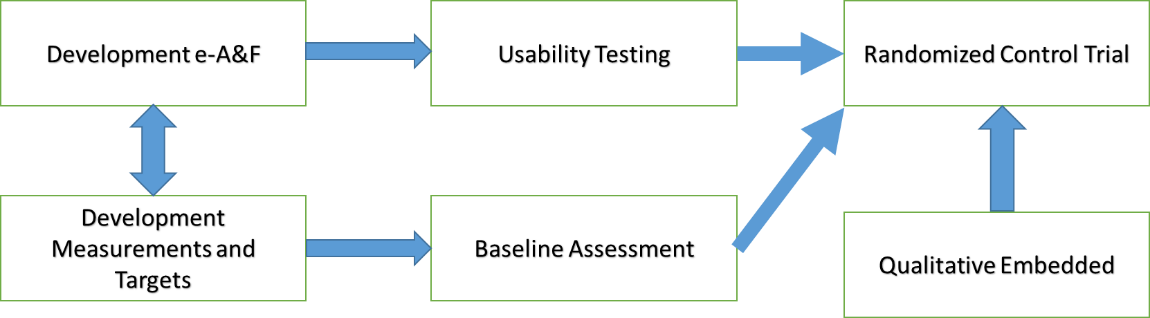
\includegraphics[width=\textwidth]{img/overall_sequence.png}
    \caption{Overall sequence, research project}
    \label{fig:ove_seq}
\end{figure}

The participants will be physicians and trainees from the participating department. Informed consent will be obtained and participants can step out at any time. Performance feedback will be confidential and personal. No clinical data will be captured specifically for this project, only secondary data will be used. The A\&F system will leverage the MUHC data warehouse to automate data collection.

\begin{figure}[h]
    \centering
    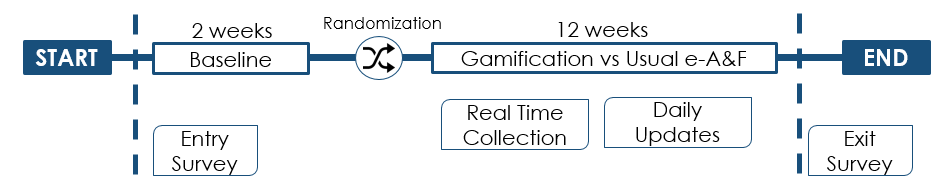
\includegraphics[width=\textwidth]{img/rct_flow.png}
    \caption{Diagram of the RCT process}
    \label{fig:rct_flow}
\end{figure}

\subsubsection{Participants}
* Attending Physicians, Residents (Cardiology, and others), Fellow

Physicians of the cardiology ward, at the MUHC Glen hospital.

Includes : Attending physicians, residents (IM and others), fellows
Eligibility : At least one month as part of the IM ward
Locations : Single Centre
Characteristics : 
Highly educated
Limited Time
Spectrum of ages
Variable IT familiarity


\subsubsection{Recruitment and Consent}
* Recruitment plans and consent process

\subsubsection{Randomization Method and Blinding}
== Randomization

Stratification levels : Attendings / Residents

Chosen randomly (by the system) after a user logs in with their user type.

Anonymous ID is created and associated with user profile in secure DB.

Randomization will likely be imbalanced on some aspects due to low Ns.


== Blinding

Blinding researchers but not participants

Participants can’t be blinded to this

Researcher can since data is collected automatically using anonymous IDs

Analysis can be blinded by not knowing which group is which.

Baseline questionnaires are taken before participants are randomized.


\subsubsection{Data Collection}
\lipsum[2]

\subsubsection{Risks and Benefits?}
Needs plan to prevent rejection, lack of trust, or perceived intrusion

\lipsum[1]

\subsubsection{Withdrawal of Subjects}

Participants can stop using their assigned system at anytime, but they won't be allowed access to the other branch. If participants either want to leave the study, or expect they won't handle case in this department anymore, an exit questionnaire will be given at that time.


\lipsum[1]

\subsubsection{Interventions}
Individual confidential Web-based portal, delivered through navigating to a specific URL on a ward computer or personal device.
No ready made public base e-A\&F to compare (and would be difficult)
Gamification is difficult to isolate (more of an emphasis then new feature)
Difficult to consider perfect fair comparison in this case, because different in many respects and no clear guidelines on what is a base e-A\&F. (specific feat. List with demo/screen will be made)
Groups will receive the same amount, and kind of implementation effort.
Support staff on hand for both solutions,  reported Severe bugs, and potential adverse effects will be fixed during trial.

\subsubsection{Measures and Outcomes}

\textbf{Entry Questionnaire}
Basic demographic questionnaire

Technology Assessment Model v3 (v1 1989, v3 2008) validated and std.
Based on Theory of Reasoned Action
Deals with Perceived Ease of Use and Perceived Usefulness
Sub. Cri. : Computer Anxiety, Comp. Playfulness, Comp. Self-Efficacy, external control.
Known confounder of IT use and effective use.

\textbf{Main Measures}
Primary
Adoption (as count of login <= 30 days)
Sustained Use (as login rates > 30 days)
Not standardized, most are marketing metrics.

Performance targets, as defined by the A\&F committee.
Likely continuous measure for 1) DM care and 2) antimicrobial use
All process measures

\textbf{Exit Questionnaire}
Something that matches our behaviour change framework?


\begin{itemize}
    \item Adoption \\ How is it measured?
    \item Engagement \\ How is it measured?
    \item Effectiveness (EMM?) \\ How is it measured?
\end{itemize}

\subsubsection{Statistical Plan}

Two arm, parallel design, individual RCT using a intention to treat (ITT) approach.

Cross-over might not be appropriate due to concerns of carryover effects.

(There will be no stop rule, due to the difficulty of finding good prior)

Bayesian sample size analysis, using priors from past study on adoption and sustained use.

Average Length Criteria to ensure for the comparison of credible intervals

Including priors on participation rates

We will used bayesian missing data technique to predict missing data on the TAMv3 and demographic baseline questionnaires.

Comparison of overlapping credible intervals for 
	counts in adoption 
	rates for sustainability
	proportions in the performance measures

Using same priors for adoption and sustain used
adjusting for any unbalanced confounders (age, sex, TAM)
Controlling for their strata



\textbf{Sample Size / Power}
Everyone? How many is everyone. Can we do a quick test to see how close will this be to sufficient?
Difficulty in putting a clinical meaningfulness threshold?

\textbf{Missing Data}
Stuff

\subsection{Qualitative Embedded}

\begin{itemize}
    \item Participants Impression of Gamification
    \item Elicitation of Adverse Perception?
    \item Getting more info on perception of whether gamification was useful.
    \item Adequacy of the targets
    \item Impact on social interactions
    \item Mode of Resolving feedback-self discrepancies (incl. self-efficacy)
\end{itemize}

\subsubsection{Ethical Considerations}
Performance feedback is confidential, and won’ t be shared (unless required by law)


* Taking time away from patient treatment/asking for doctor's time outside of work hours?
* Informed consent will be required from all participants, but not from patients.

-- ?
* Saying something medical, possibly opposite?


\subsection{Data Handling}
Confidentiality, Security, and Records Retention, + Public Reporting?

* Patient data will not be kept in the system, deanonymized participants metrics will be published along with the publication, and code?
* Nominalized patients data is used for the feedback, but anonymized physician IDs with metrics

Secure server, (watched 24/7 locked door and keycard). Data will reside on central server or analysis cluster. With researchers being forbidden to download the data on their local computers.

Link between anonymous ID and participants ID will be stored securely on the same server.
